\chapter{Thermal conductivity simulations of Silica glass}

\LEnote{*** INTRODUCTION, STATO DELL'ARTE ***}

%%%%%%%%%%%%%%%%%%%%%%%%%%%%%%%%%%%%%%%%%%%%%
\section{Classical simulations: sample}

\subsection{Force field}
BKS
\begin{figure}
    \centering
    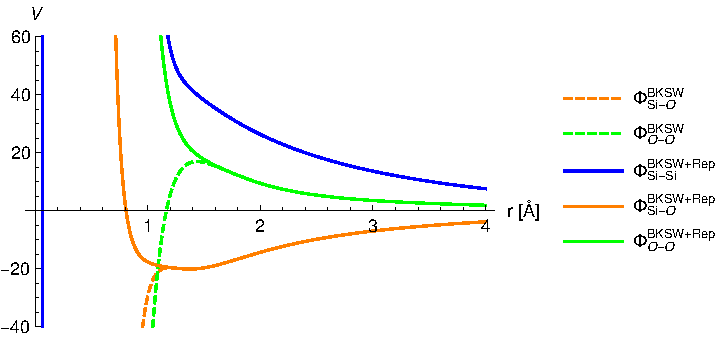
\includegraphics[]{chapters/chapter6/figures/BKSW.pdf}
    \caption{BKS potential with Wolf truncation.}
    \label{fig:BKS-potential}
\end{figure}

\subsection{Sample preparation}

\subsection{Quenching}

%%%%%%%%%%%%%%%%%%%%%%%%%%%%%%%%%%%%%%%%%%%%%
\section{Classical simulations: thermal conductivity}

\subsection{Cepstral analysis}
\paragraph{Dependence on cutoff frequency $f^*$}
(For the chosen sample at experimental density)
(comparison bw normal and vel-renormalized results)

\begin{figure}
    \centering
    \subfigure[\label{fig:csilica-sample-expdens-fstar-100ps}]{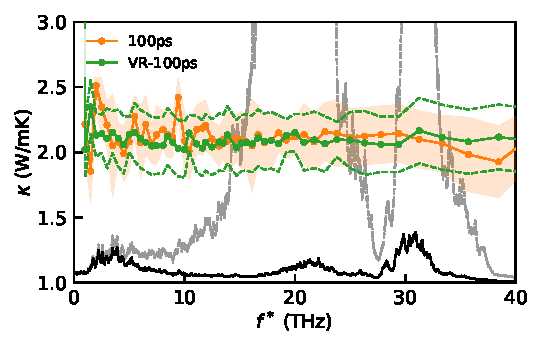
\includegraphics[width=8cm]{chapters/chapter6/figures/silica_expdens_kappa_fstar_VR_100ps.pdf}}
    \subfigure[\label{fig:csilica-sample-expdens-fstar-1ns}]{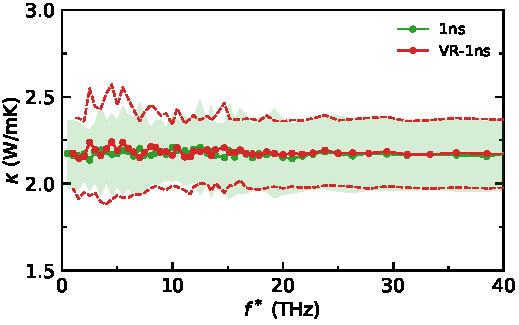
\includegraphics[width=8cm]{chapters/chapter6/figures/silica_expdens_kappa_fstar_VR_1ns.pdf}}
    \subfigure[\label{fig:csilica-sample-expdens-fstar-10ns}]{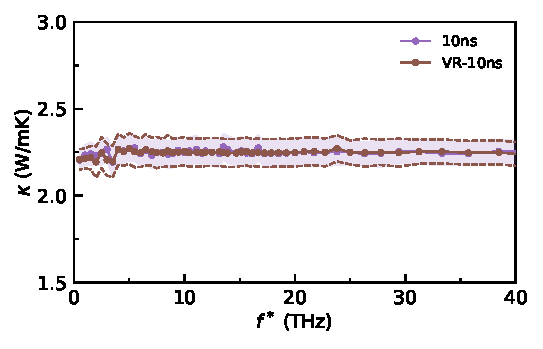
\includegraphics[width=8cm]{chapters/chapter6/figures/silica_expdens_kappa_fstar_VR_10ns.pdf}}
    \caption{Dependence of $\kappa$ on the choice of the cutoff frequency $f^*$, estimated from \emph{one} sample of (a) $100\un{ps}$, (b) $1\un{ns}$, and (c) $10\un{ps}$ of the ``original'' and VR heat flux time series. 
    The original and VR periodograms are reported for reference with grey and black lines, respectively.}
    \label{fig:csilica-sample-expdens-fstar}
\end{figure}
Fig.~\ref{fig:csilica-sample-expdens-fstar} -- stability of $\kappa$ as a function of $f^*$ increases with the length of the trajectory, as its predicted error decreases. The values and errors of $\kappa$ obtained from the VR time series are equivalent to the ones obtained from the original time series, and are slightly more stable with $f^*$. This is probably due to the much smaller power of the power spectrum of the VR heat flux, that may decrease the small artifacts introduced by the low-pass filter applied before resampling. 
Any frequency in the central region of the spectrum can be taken as $f^*$, hence we choose to set $f^*=28\un{THz}$. Conversely, a $f^*$ too small makes $\kappa$ deviate sensibly, due to the fact that the low-pass filter is not strong enough to avoid aliasing effects that modify the spectrum of the resampled time series; instead, a $f^*$ that is too high ($f^*\gtrsim 60\un{THz}$) induces a bias in $\kappa$, due to the fact the log-periodogram diverges to negative values and we start to have problems of numerical precision.

